\documentclass[11pt,a4paper]{article}

% --- Packages ---
\usepackage[utf8]{inputenc}
\usepackage[T1]{fontenc}
\usepackage{lmodern} 
\usepackage[margin=1in, headheight=14pt]{geometry} 
\usepackage{titlesec}
\usepackage{titletoc}
\usepackage{fancyhdr}
\usepackage{graphicx} 
\usepackage{booktabs} 
\usepackage{longtable}
\usepackage{array}
\usepackage{enumitem} 
\usepackage{float}
\usepackage{listings}
\usepackage{xcolor}
\usepackage{tikz}
\usetikzlibrary{shapes, arrows.meta, positioning, fit, backgrounds, calc, shadows, trees}
\usepackage{amssymb} 
\usepackage{xurl} 
\usepackage[hidelinks]{hyperref}

% --- Typography & Layout ---
\hypersetup{
    colorlinks=false,
    pdftitle={Architecture Decision Record: Git CMS},
    pdfauthor={James Ross}
}

\usepackage{parskip}
\setlength{\parindent}{0pt}
\setlength{\parskip}{0.8em}

\pagestyle{fancy}
\fancyhf{}
\fancyhead[L]{\nouppercase{\leftmark}}
\fancyhead[R]{Git CMS ADR}
\fancyfoot[C]{\thepage}

\titleformat{\section}{\Large\bfseries\sffamily}{\thesection}{1em}{}
\titleformat{\subsection}{\large\bfseries\sffamily}{\thesubsection}{1em}{}
\titleformat{\subsubsection}{\bfseries\sffamily}{\thesubsubsection}{1em}{}

\lstset{
    basicstyle=\ttfamily\small,
    breaklines=true,
    frame=single, 
    numbers=left,
    numberstyle=\tiny\color{gray},
    captionpos=b,
    keepspaces=true,
    showstringspaces=false,
    keywordstyle=\bfseries, 
    commentstyle=\itshape,  
    stringstyle=,           
}

% --- Textbook B&W TikZ Styles ---
\tikzset{
    base/.style={draw=black, thick, font=\sffamily\small, align=center, inner sep=8pt},
    block/.style={base, rectangle, rounded corners=2pt, fill=white},
    blockshaded/.style={base, rectangle, rounded corners=2pt, fill=gray!10},
    line/.style={draw=black, thick, -Latex},
    dashed-line/.style={draw=black, thick, dashed, -Latex}
}

\begin{document}

% meta.tex
\title{Architecture Decision Record: Git CMS\\ \large Database-Free Content Management via Git Plumbing}
\author{James Ross}
\date{Version 1.0.0 \textemdash{} Last Updated: \today}


\begin{titlepage}
    \centering
    \vspace*{3cm}
    {\fontsize{30}{36}\selectfont \textbf{Architecture Decision Record}\\[0.5em]}
    {\fontsize{20}{24}\selectfont \textit{Git CMS}\\[1.5cm]}
    
    \rule{\textwidth}{1pt}\\[0.5cm]
    {\Large Database-Free Content Management via Git Plumbing}\\[3cm]
    
    \textbf{Author:} James Ross \\
    \textbf{Version:} 1.0.0 \\
    \textbf{Date:} 2026-01-11
    
    \vfill
    \textit{Prepared for Engineering Review}
    \vspace{2cm}
\end{titlepage}

\tableofcontents
\newpage

\section{Introduction \& Goals}

\subsection{Project Overview}

\textbf{git-cms} is a serverless, database-free Content Management System that treats Git's object store as a distributed, cryptographically verifiable document database. Instead of storing content in traditional databases (SQL or NoSQL), it leverages Git's Merkle DAG to create an append-only ledger for articles, metadata, and encrypted assets.

The fundamental innovation: \texttt{git push} becomes the API endpoint.

\subsection{Fundamental Requirements}

\subsubsection{FR-1: Zero-Database Architecture}
\label{fr:zero-database}
The system MUST NOT depend on external database systems (SQL, NoSQL, or key-value stores). All persistent state resides within Git's native object store (\texttt{.git/objects}).

\textbf{Rationale:} Eliminates operational complexity, deployment dependencies, and schema migration challenges inherent to traditional database-backed CMSs.

\subsubsection{FR-2: Cryptographic Verifiability}
\label{fr:crypto-verify}
Every content mutation MUST be recorded as a Git commit with cryptographic integrity guarantees via Git object hashing (SHA-1 in default mode; SHA-256 in SHA-256 repositories) and optional GPG signing for non-repudiation. SHA-1 collision weaknesses are acknowledged; migration to SHA-256 object format is the target state as tooling matures.

\textbf{Rationale:} Provides immutable audit trails and tamper detection without additional infrastructure.

\subsubsection{FR-3: Fast-Forward Only Publishing}
\label{fr:fast-forward-publish}
The publish operation MUST enforce strict linear history (fast-forward only) to prevent rewriting published content.

\textbf{Rationale:} Guarantees provenance and prevents content manipulation after publication.

\subsubsection{FR-4: Client-Side Encryption}
\label{fr:client-encryption}
All uploaded assets MUST be encrypted client-side (AES-256-GCM) before touching the repository.

\textbf{Rationale:} Achieves row-level security without database-level access controls. The Git gateway receives only opaque encrypted blobs.

\subsubsection{FR-5: Infinite Point-in-Time Recovery}
\label{fr:infinite-recovery}
Users MUST be able to access any historical version of any article without data loss.

\textbf{Rationale:} Git's DAG structure provides this naturally; the CMS simply exposes it as a first-class feature.

\subsection{Quality Goals}

\begin{table}[H]
\centering
\small
\begin{tabular}{llp{5cm}p{4cm}}
\toprule
\textbf{Prio} & \textbf{Attribute} & \textbf{Description} & \textbf{Measurement} \\
\midrule
1 & Security & Cryptographic integrity, signed commits & GPG verification, AES-256 strength \\
2 & Simplicity & Minimal dependencies, composable architecture & Lines of code, dependency count \\
3 & Auditability & Complete provenance of all content changes & Git log completeness \\
4 & Performance & Sub-second reads for blog workloads & Response time for \texttt{readArticle()} \\
5 & Portability & Multi-runtime support (Node, Bun, Deno) & Test suite pass rate \\
\bottomrule
\end{tabular}
\caption{Quality goals and their measurements.}
\end{table}

\subsection{Non-Goals}

This system is \textbf{intentionally NOT designed for}:

\begin{itemize}[noitemsep]
    \item \textbf{High-velocity writes:} Content publishing happens in minutes/hours, not milliseconds.
    \item \textbf{Complex queries:} No SQL-like JOINs or aggregations. Queries are limited to ref enumeration and commit message parsing.
    \item \textbf{Large-scale collaboration:} Designed for single-author or small-team blogs.
    \item \textbf{Real-time updates:} Publishing is atomic but not instantaneous.
\end{itemize}

\section{Constraints}

\subsection{Technical Constraints}

\textbf{TC-1: Git's Content Addressability Model} \\
Git uses SHA-1 hashing for object addressing. While SHA-1 has known collision vulnerabilities, Git is transitioning to SHA-256. The system assumes SHA-1 is ``good enough'' for content addressing (not for security-critical signing).

\textbf{Mitigation:} Use GPG signing (\texttt{CMS\_SIGN=1}) for cryptographic non-repudiation.

\textbf{TC-2: Filesystem I/O Performance} \\
All Git operations are ultimately filesystem operations. Performance is bounded by disk I/O, especially for large repositories.

\textbf{Mitigation:} Content is stored as commit messages (small), not files (large). Asset chunking (256KB) reduces blob size.

\textbf{TC-3: POSIX Shell Dependency} \\
The \texttt{@git-stunts/plumbing} module executes Git via shell commands (\texttt{child\_process.spawn}). This requires a POSIX-compliant shell and Git CLI.

\textbf{Mitigation:} All tests run in Docker (Alpine Linux) to ensure consistent environments.

\textbf{TC-4: No Database Indexes} \\
Traditional databases provide B-tree indexes for fast lookups. Git's ref enumeration is linear (\texttt{O(n)} for listing all refs in a namespace).

\textbf{Mitigation:} Use ref namespaces strategically (e.g., \texttt{refs/\_blog/articles/<slug>}) to avoid polluting the global ref space.

\subsection{Regulatory Constraints}

\textbf{RC-1: GDPR Right to Erasure} \\
Git's immutability conflicts with GDPR's ``right to be forgotten.'' Deleting a commit requires rewriting history, which breaks cryptographic integrity.

\textbf{Mitigation:} Use encrypted assets with key rotation. Deleting the encryption key renders historical content unreadable without altering Git history.

\textbf{RC-2: Cryptographic Export Restrictions} \\
AES-256-GCM encryption may face export restrictions in certain jurisdictions.

\textbf{Mitigation:} The \texttt{@git-stunts/vault} module uses Node's built-in \texttt{crypto} module, which is widely available.

\subsection{Operational Constraints}

\textbf{OC-1: Single-Writer Assumption} \\
Git's ref updates are atomic \textit{locally} but not across distributed clones. Concurrent writes to the same ref can cause conflicts.

\textbf{Mitigation:} Use \textbf{git-stargate} (a companion project) to enforce serialized writes via SSH.

\textbf{OC-2: Repository Growth} \\
Every draft save creates a new commit. Repositories can grow unbounded over time.

\textbf{Mitigation:} Use \texttt{git gc} aggressively. Consider ref pruning for old drafts.
\section{Context \& Scope}

\subsection{System Context Diagram}

\begin{figure}[H]
\centering
\resizebox{\textwidth}{!}{
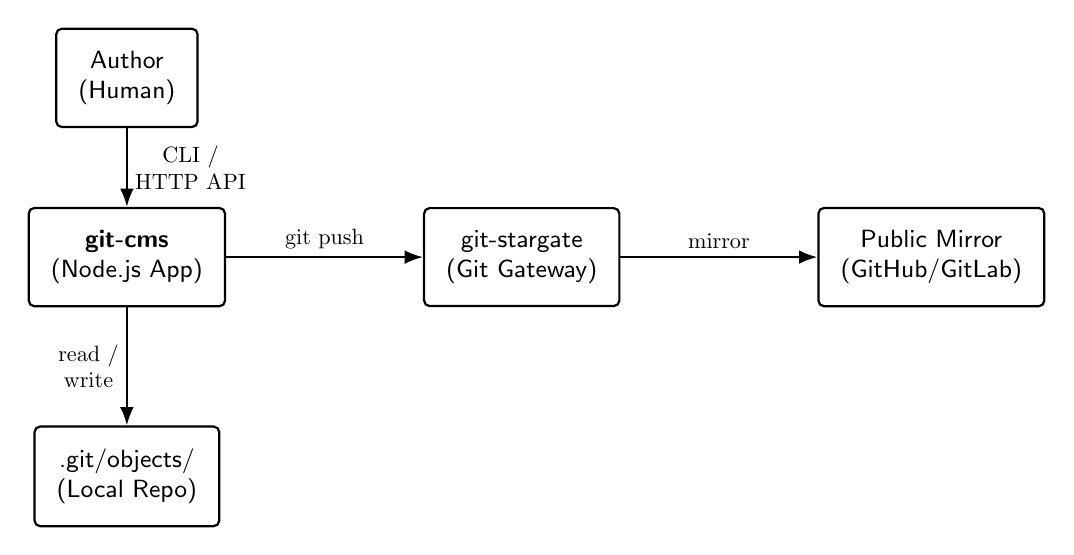
\begin{tikzpicture}[node distance=2cm, auto]
    \node [block] (Author) {Author\\(Human)};
    \node [block, below=1cm of Author] (GitCMS) {\textbf{git-cms}\\(Node.js App)};
    \node [block, right=2.5cm of GitCMS] (Stargate) {git-stargate\\(Git Gateway)};
    \node [block, below=1.5cm of GitCMS] (LocalRepo) {.git/objects/\\(Local Repo)};
    \node [block, right=2.5cm of Stargate] (PublicMirror) {Public Mirror\\(GitHub/GitLab)};

    \path [line] (Author) -- node [align=center, scale=0.8] {CLI /\\ HTTP API} (GitCMS);
    \path [line] (GitCMS) -- node [align=center, scale=0.8] {git push} (Stargate);
    \path [line] (GitCMS) -- node [align=center, scale=0.8, swap] {read /\\ write} (LocalRepo);
    \path [line] (Stargate) -- node [align=center, scale=0.8] {mirror} (PublicMirror);
\end{tikzpicture}
}
\caption{System context diagram showing the high-level relationship between the Author, Git CMS, and external components.}
\end{figure}

\subsection{External Interfaces}

\subsubsection{Interface 1: CLI (Binary)}
\begin{itemize}[noitemsep]
    \item \textbf{Entry Point:} \texttt{bin/git-cms.js}
    \item \textbf{Commands:} \texttt{draft}, \texttt{publish}, \texttt{list}, \texttt{show}, \texttt{serve}
    \item \textbf{Protocol:} POSIX command-line arguments
    \item \textbf{Example:}
\end{itemize}

\begin{lstlisting}[language=bash]
echo "# Hello World" | git cms draft hello-world "My First Post"
\end{lstlisting}

\subsubsection{Interface 2: HTTP API (REST)}
\begin{itemize}[noitemsep]
    \item \textbf{Server:} \texttt{src/server/index.js}
    \item \textbf{Port:} 4638 (configurable via \texttt{PORT} env var)
    \item \textbf{Endpoints:}
    \begin{itemize}[noitemsep]
        \item \texttt{POST /api/cms/snapshot} -- Save draft
        \item \texttt{POST /api/cms/publish} -- Publish article
        \item \texttt{GET /api/cms/list} -- List articles
        \item \texttt{GET /api/cms/show?slug=<slug>} -- Read article
    \end{itemize}
    \item \textbf{Authentication:} None (assumes private network or SSH tunneling). \textit{See Section 11 (Risks) for threat-model implications and mitigations.}
\end{itemize}

\subsubsection{Interface 3: Git Plumbing (Shell)}
\begin{itemize}[noitemsep]
    \item \textbf{Protocol:} Git CLI commands via \texttt{child\_process.spawn}
    \item \textbf{Critical Commands:}
    \begin{itemize}[noitemsep]
        \item \texttt{git commit-tree} -- Create commits on empty trees
        \item \texttt{git update-ref} -- Atomic ref updates
        \item \texttt{git for-each-ref} -- List refs in namespace
        \item \texttt{git cat-file} -- Read commit messages
    \end{itemize}
\end{itemize}

\subsubsection{Interface 4: OS Keychain (Secrets)}
\begin{itemize}[noitemsep]
    \item \textbf{Platforms:}
    \begin{itemize}[noitemsep]
        \item macOS: \texttt{security} tool
        \item Linux: \texttt{secret-tool} (GNOME Keyring)
        \item Windows: \texttt{CredentialManager} (PowerShell)
    \end{itemize}
    \item \textbf{Purpose:} Store AES-256-GCM encryption keys for assets
\end{itemize}

\subsection{Scope Boundaries}

\subsubsection{In Scope}
\begin{itemize}[noitemsep]
    \item Article drafting, editing, and publishing
    \item Encrypted asset storage (images, PDFs)
    \item Full version history via Git log
    \item CLI and HTTP API access
    \item Multi-runtime support (Node, Bun, Deno)
\end{itemize}

\subsubsection{Out of Scope}
\begin{itemize}[noitemsep]
    \item \textbf{User Authentication:} Delegated to git-stargate or SSH
    \item \textbf{Search Indexing:} No full-text search (external indexer required)
    \item \textbf{Media Transcoding:} Assets stored as-is
    \item \textbf{Real-Time Collaboration:} No OT or CRDTs
    \item \textbf{Analytics:} No built-in tracking
\end{itemize}

\section{Solution Strategy}

\subsection{Core Architectural Principles}

\paragraph{P-1: Composition over Inheritance}
The system is built from \textbf{five independent Lego Block modules} (\texttt{@git-stunts/*}), each with a single responsibility. These modules are composed in \texttt{CmsService} to create higher-order functionality.

\textbf{Benefit:} Each module can be tested, versioned, and published independently.

\paragraph{P-2: Hexagonal Architecture (Ports \& Adapters)}
The domain layer (\texttt{CmsService}) depends on abstractions (\texttt{GitPlumbing}, \texttt{TrailerCodec}), not implementations. This allows swapping out Git for other backends (e.g., a pure JavaScript implementation for testing).

\textbf{Benefit:} Decouples domain logic from infrastructure concerns.

\paragraph{P-3: Content Addressability}
Assets are stored by their SHA-1 hash, enabling automatic deduplication. If two articles reference the same image, it's stored once.

\textbf{Benefit:} Reduces repository bloat.

\paragraph{P-4: Cryptographic Integrity}
Every operation produces a cryptographically signed commit (when \texttt{CMS\_SIGN=1}). The Merkle DAG ensures tamper detection.

\textbf{Benefit:} Audit trails are mathematically verifiable, not just trust-based.

\subsection{Solution Approach: The \"Empty Tree\" Stunt}

\paragraph{The Problem}
Traditional CMSs store content in database rows. Git is designed to track \textit{files}, not arbitrary data. Storing blog posts as files (e.g., \texttt{posts/hello-world.md}) clutters the working directory and causes merge conflicts.

\paragraph{The Solution}
Store content as \textbf{commit messages on empty trees}, not as files. Every article is a commit that points to the well-known empty tree (\texttt{4b825dc642cb6eb9a060e54bf8d69288fbee4904}).

\textbf{How It Works:}
\begin{enumerate}[noitemsep]
    \item Encode the article (title, body, metadata) into a Git commit message using RFC 822 trailers.
    \item Create a commit that points to the empty tree (no files touched).
    \item Update a ref (e.g., \texttt{refs/\_blog/articles/hello-world}) to point to this commit.
\end{enumerate}

\textbf{Result:} The repository's working directory remains clean. All content lives in \texttt{.git/objects/} and \texttt{.git/refs/}.

\paragraph{Architectural Pattern: Event Sourcing}
Each draft save creates a new commit. The \"current\" article is the ref's tip, but the full history is a linked list of commits.

\textbf{Benefit:} Point-in-time recovery is trivial (\texttt{git log refs/\_blog/articles/<slug>}).

\subsection{Key Design Decisions}

\paragraph{D-1: Why Commit Messages, Not Blobs?}
\textbf{Alternative:} Store articles as Git blobs and reference them via trees. \\
\textbf{Decision:} Use commit messages. \\
\textbf{Rationale:} Commits have parent pointers (version history) and support GPG signing (non-repudiation). Blobs are opaque; messages are human-readable.

\paragraph{D-2: Why Trailers, Not JSON?}
\textbf{Alternative:} Store \texttt{\{\"title\": \"Hello\", ...\}} as the message. \\
\textbf{Decision:} Use RFC 822 trailers. \\
\textbf{Rationale:} Trailers are Git-native, human-readable, and diff-friendly. Backward parsing is efficient.

\paragraph{D-3: Why Encrypt Assets, Not Repos?}
\textbf{Alternative:} Use \texttt{git-crypt} for the whole repo. \\
\textbf{Decision:} Encrypt individual assets client-side. \\
\textbf{Rationale:} Granular control; the gateway never sees plaintext.
\section{Building Block View}

\subsection{Level 1: System Decomposition}

\begin{figure}[H]
\centering
\resizebox{\textwidth}{!}{
    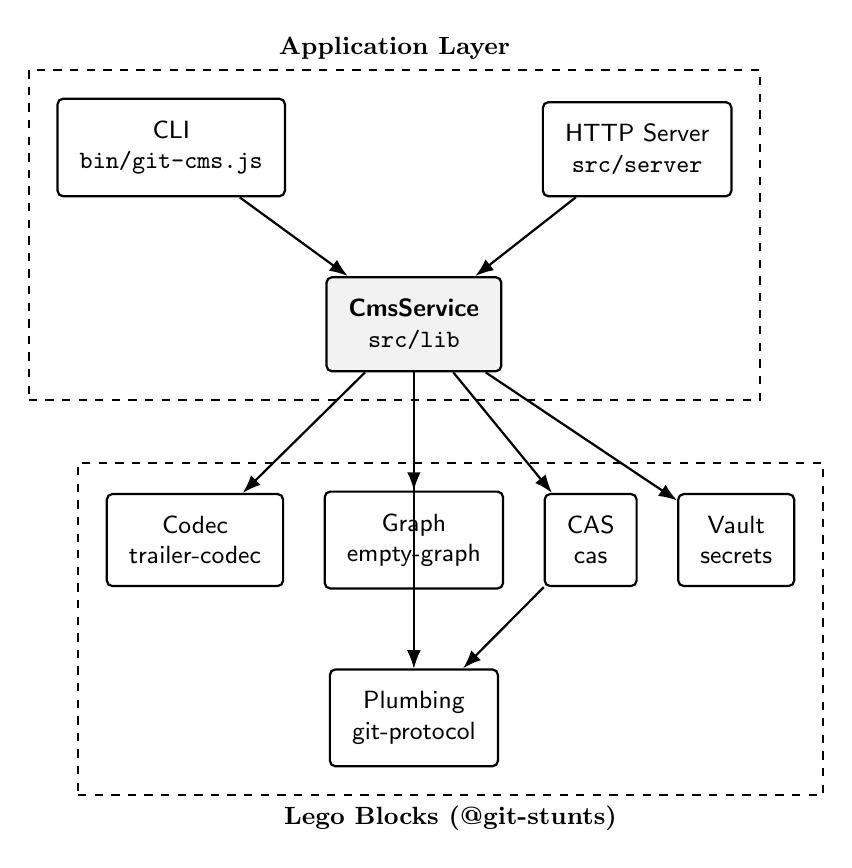
\begin{tikzpicture}[node distance=1.5cm, auto]
    \node [blockshaded] (CMS) {\textbf{CmsService}\\\texttt{src/lib}};
    \node [block, above left=1cm and 0.5cm of CMS] (CLI) {CLI\\\texttt{bin/git-cms.js}};
    \node [block, above right=1cm and 0.5cm of CMS] (HTTP) {HTTP Server\\\texttt{src/server}};
    \node [draw, dashed, thick, inner sep=10pt, fit=(CLI) (HTTP) (CMS)] (AppLayer) {};
    \node [anchor=south] at (AppLayer.north) {\small\textbf{Application Layer}};

    \node [block, below=1.5cm of CMS] (Graph) {Graph\\empty-graph};
    \node [block, left=0.5cm of Graph] (Codec) {Codec\\trailer-codec};
    \node [block, right=0.5cm of Graph] (CAS) {CAS\\cas};
    \node [block, below=1cm of Graph] (Plumbing) {Plumbing\\git-protocol};
    \node [block, right=0.5cm of CAS] (Vault) {Vault\\secrets};
    \node [draw, dashed, thick, inner sep=10pt, fit=(Plumbing) (Codec) (Graph) (CAS) (Vault)] (LegoLayer) {};
    \node [anchor=north] at (LegoLayer.south) {\small\textbf{Lego Blocks (@git-stunts)}};

    \draw [line] (CLI) -- (CMS); \draw [line] (HTTP) -- (CMS);
    \draw [line] (CMS) -- (Codec); \draw [line] (CMS) -- (Graph);
    \draw [line] (CMS) -- (CAS); \draw [line] (CMS) -- (Vault);
    \draw [line] (CMS) -- (Plumbing); \draw [line] (Graph) -- (Plumbing);
    \draw [line] (CAS) -- (Plumbing);
\end{tikzpicture}
}
\caption{System decomposition showing the interaction between the application layer and the independent Lego block modules.}
\end{figure}

\subsection{Level 2: Lego Block Responsibilities}

\begin{figure}[H]
\centering
\resizebox{\textwidth}{!}{
    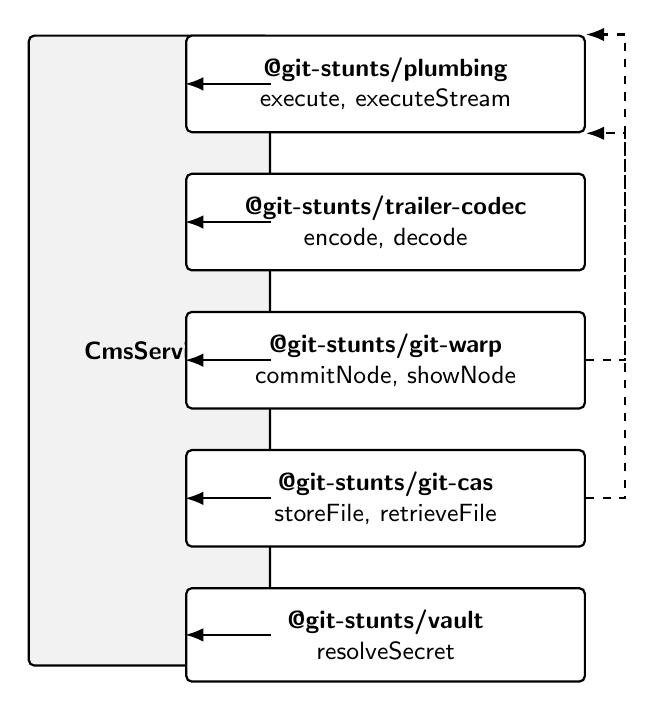
\begin{tikzpicture}[auto, font=\small]
    \node [blockshaded, text width=2.5cm, minimum height=8cm] (CMS) {\textbf{CmsService}};
    \node [block, text width=4.5cm, right=3cm of CMS.north, anchor=north] (PL) {\textbf{@git-stunts/plumbing}\\execute, executeStream};
    \node [block, text width=4.5cm, below=0.5cm of PL] (TC) {\textbf{@git-stunts/trailer-codec}\\encode, decode};
    \node [block, text width=4.5cm, below=0.5cm of TC] (EG) {\textbf{@git-stunts/git-warp}\\commitNode, showNode};
    \node [block, text width=4.5cm, below=0.5cm of EG] (CAS) {\textbf{@git-stunts/git-cas}\\storeFile, retrieveFile};
    \node [block, text width=4.5cm, below=0.5cm of CAS] (V) {\textbf{@git-stunts/vault}\\resolveSecret};

    \draw [line] (CMS.east |- PL.west) -- (PL.west);
    \draw [line] (CMS.east |- TC.west) -- (TC.west);
    \draw [line] (CMS.east |- EG.west) -- (EG.west);
    \draw [line] (CMS.east |- CAS.west) -- (CAS.west);
    \draw [line] (CMS.east |- V.west) -- (V.west);

    \draw [dashed-line] (EG.east) -- ++(0.5,0) |- (PL.north east);
    \draw [dashed-line] (CAS.east) -- ++(0.5,0) |- (PL.south east);
\end{tikzpicture}

}
\caption{Detailed responsibilities and API surfaces of the Git CMS modules.}
\end{figure}
\section{Runtime View}

\subsection{Scenario 1: Create Draft Article}

\begin{figure}[H]
\centering
\resizebox{\textwidth}{!}{
    \begin{tikzpicture}[node distance=3cm, auto]
    \node (Author) {Author};
    \node [right=of Author] (CLI) {CLI};
    \node [right=of CLI] (CMS) {Service};
    \node [right=of CMS] (PL) {Plumbing};

    \foreach \n in {Author, CLI, CMS, PL} {
        \draw [dashed] (\n) -- ++(0,-6.5);
    }

    \draw [->] ($(Author)+(0,-1)$) -- node [scale=0.7] {draft hello-world} ($(CLI)+(0,-1)$);
    \draw [->] ($(CLI)+(0,-1.5)$) -- node [scale=0.7] {saveSnapshot()} ($(CMS)+(0,-1.5)$);
    \draw [->] ($(CMS)+(0,-2.2)$) -- node [scale=0.7] {revParse(ref)} ($(PL)+(0,-2.2)$);
    \draw [<-] ($(CMS)+(0,-3)$) -- node [scale=0.7] {null} ($(PL)+(0,-3)$);
    \draw [->] ($(CMS)+(0,-4)$) -- ++(1.2,0) -- ++(0,-0.6) -- ++(-1.2,0) node [scale=0.7, pos=0.55, above] {createNode()};
    \draw [->] ($(CMS)+(0,-5)$) -- node [scale=0.7] {updateRef()} ($(PL)+(0,-5)$);
    \draw [<-] ($(CLI)+(0,-6)$) -- node [scale=0.7] {OK} ($(CMS)+(0,-6)$);
\end{tikzpicture}

}
\caption{Sequence diagram for creating a new draft article.}
\end{figure}

\subsection{Scenario 2: Publish Article}
Publishing is \textbf{just a ref copy}. No new commits are created. This operation is idempotent and enforces fast-forward updates.

\subsection{Scenario 3: Upload Encrypted Asset}
The system splits files into 256KB chunks, encrypts them via AES-256-GCM, and stores them as Git blobs. The plaintext never touches the object store.

\subsection{Scenario 4: List All Published Articles}
Listing articles involves a linear scan of the ref namespace (\texttt{O(n)}). For large workloads, an external index is recommended.
\section{Deployment View}

\subsection{Topology 1: Single-Author Local Blog}

\begin{figure}[H]
\centering
\resizebox{\textwidth}{!}{
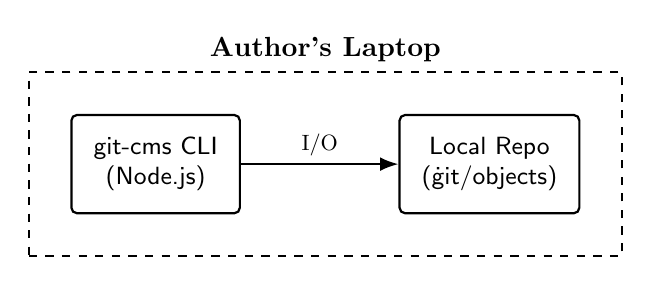
\begin{tikzpicture}
    \node [block] (CLI) {git-cms CLI\\(Node.js)};
    \node [block, right=2cm of CLI] (Repo) {Local Repo\\(\.git/objects)};
    \draw [line] (CLI) -- node [above, scale=0.8] {I/O} (Repo);
    \node [draw, dashed, thick, inner sep=15pt, fit=(CLI) (Repo)] (Box) {};
    \node [anchor=south, font=\bfseries] at (Box.north) {Author's Laptop};
\end{tikzpicture}
}
\caption{Local deployment topology.}
\end{figure}

\subsection{Topology 2: Team Blog with Stargate Gateway}

\begin{figure}[H]
\centering
\resizebox{\textwidth}{!}{
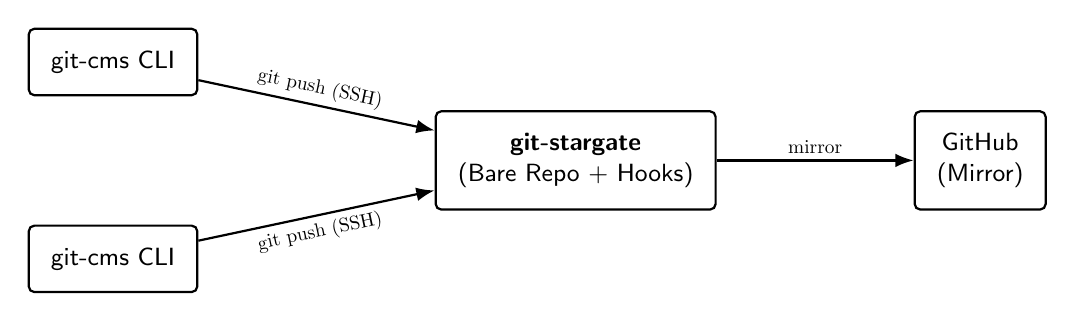
\begin{tikzpicture}[node distance=2.5cm]
    \node [block] (CMS_A) {git-cms CLI};
    \node [block, below of=CMS_A] (CMS_B) {git-cms CLI};
    \node [block, right=3cm of CMS_A, yshift=-1.25cm] (Stargate) {\textbf{git-stargate}\\(Bare Repo + Hooks)};
    \node [block, right=2.5cm of Stargate] (GitHub) {GitHub\\(Mirror)};

    \draw [line] (CMS_A) -- node [above, sloped, scale=0.7] {git push (SSH)} (Stargate);
    \draw [line] (CMS_B) -- node [below, sloped, scale=0.7] {git push (SSH)} (Stargate);
    \draw [line] (Stargate) -- node [above, scale=0.7] {mirror} (GitHub);
\end{tikzpicture}
}
\caption{Collaborative deployment topology using a central gateway.}
\end{figure}

\subsection{Topology 3: Dockerized Development}

\begin{figure}[H]
\centering
\resizebox{\textwidth}{!}{
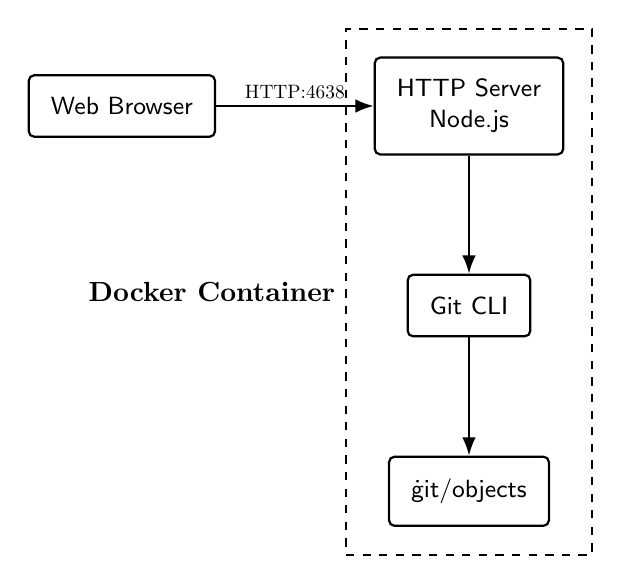
\begin{tikzpicture}[node distance=1.5cm]
    \node [block] (Node) {HTTP Server\\Node.js};
    \node [block, below=of Node] (Git) {Git CLI};
    \node [block, below=of Git] (Repo) {\.git/objects};
    
    \node [draw, dashed, thick, inner sep=10pt, fit=(Node) (Git) (Repo)] (Cont) {};
    \node [anchor=east, font=\bfseries] at (Cont.west) {Docker Container};
    
    \node [block, left=2cm of Node] (Browser) {Web Browser};
    \draw [line] (Browser) -- node [above, scale=0.7] {HTTP:4638} (Node);
    \draw [line] (Node) -- (Git);
    \draw [line] (Git) -- (Repo);
\end{tikzpicture}
}
\caption{Dockerized development topology.}
\end{figure}

\section{Crosscutting Concepts}

\subsection{Concept 1: Merkle DAG as Event Log}

\begin{figure}[H]
\centering
\resizebox{\textwidth}{!}{
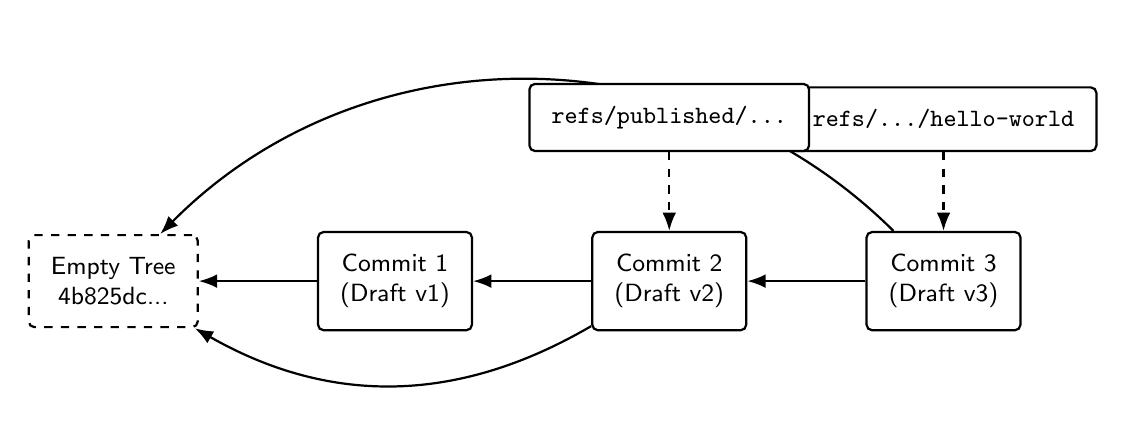
\begin{tikzpicture}[node distance=1.5cm, auto]
    \node [block, dashed] (Empty) {Empty Tree\\4b825dc...};
    \node [block, right=of Empty] (C1) {Commit 1\\(Draft v1)};
    \node [block, right=of C1] (C2) {Commit 2\\(Draft v2)};
    \node [block, right=of C2] (C3) {Commit 3\\(Draft v3)};

    \draw [line] (C1) -- (Empty);
    \draw [line] (C2) -- (C1);
    \draw [line] (C2) to [bend left=30] (Empty);
    \draw [line] (C3) -- (C2);
    \draw [line] (C3) to [bend right=45] (Empty);
    
    \node [block, above=1cm of C3] (DraftRef) {\texttt{refs/.../hello-world}};
    \node [block, above=1cm of C2] (PubRef) {\texttt{refs/published/...}};
    
    \draw [dashed-line] (DraftRef) -- (C3);
    \draw [dashed-line] (PubRef) -- (C2);
\end{tikzpicture}
}
\caption{The Merkle DAG structure acting as an immutable event log.}
\end{figure}

\subsection{Concept 2: Compare-and-Swap (CAS)}
The system uses \texttt{git update-ref <ref> <newSHA> <oldSHA>} to ensure atomic updates and prevent race conditions. If the \texttt{oldSHA} has changed since it was last read, the update is rejected.

\subsection{Concept 3: Client-Side Encryption}

\begin{figure}[H]
\centering
\resizebox{\textwidth}{!}{
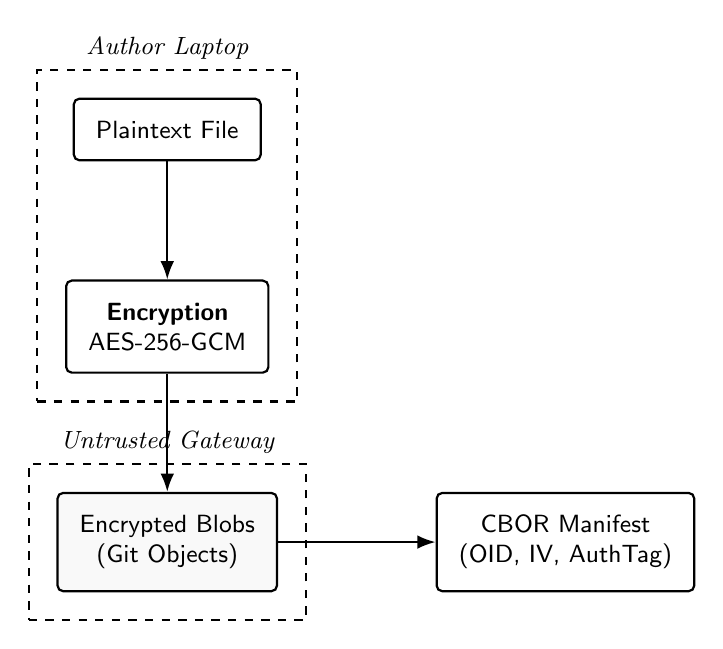
\begin{tikzpicture}[node distance=1.5cm]
    \node [block] (Input) {Plaintext File};
    \node [block, below=of Input] (Enc) {\textbf{Encryption}\\AES-256-GCM};
    \node [block, below=of Enc, fill=gray!5] (Blob) {Encrypted Blobs\\(Git Objects)};
    \node [block, right=2cm of Blob] (Manifest) {CBOR Manifest\\(OID, IV, AuthTag)};

    \draw [line] (Input) -- (Enc);
    \draw [line] (Enc) -- (Blob);
    \draw [line] (Blob) -- (Manifest);
    
    \node [draw, dashed, thick, inner sep=10pt, fit=(Input) (Enc)] (AuthorBox) {};
    \node [anchor=south, font=\small\itshape] at (AuthorBox.north) {Author Laptop};
    
    \node [draw, dashed, thick, inner sep=10pt, fit=(Blob)] (GatewayBox) {};
    \node [anchor=south, font=\small\itshape] at (GatewayBox.north) {Untrusted Gateway};
\end{tikzpicture}
}
\caption{End-to-end encryption pipeline for assets.}
\end{figure}

\section{Architectural Decisions}

\subsection*{ADR-001: Use Commit Messages, Not Files}
\textbf{Context:} Need to store articles in Git without polluting the working directory or causing merge conflicts on files.

\textbf{Decision:} Store article content (title, body, trailers) as Git commit messages pointing to the canonical empty tree (\texttt{4b825dc...}).

\textbf{Rationale:}
\begin{itemize}[noitemsep]
    \item Commits have parent pointers, enabling native version history.
    \item Commits support GPG signing for non-repudiation.
    \item Keeps the working directory completely clean for application code.
\end{itemize}

\textbf{Status:} Accepted.

\subsection*{ADR-002: Use RFC 822 Trailers, Not JSON}
\textbf{Context:} Need structured metadata (Status, Author, etc.) inside commit messages.

\textbf{Decision:} Use RFC 822 trailers (key-value pairs at the end of the message).

\textbf{Rationale:}
\begin{itemize}[noitemsep]
    \item Git-native format (compatible with \texttt{git interpret-trailers}).
    \item Human-readable and extremely diff-friendly.
    \item Faster to parse from the end of the message.
\end{itemize}

\textbf{Status:} Accepted.

\subsection*{ADR-003: Fast-Forward Only Publishing}
\textbf{Context:} Prevent published content from being altered or rewritten after release.

\textbf{Decision:} The publishing operation must be a strict fast-forward from the draft ref to the published ref.

\textbf{Rationale:} Guarantees that the exact same commit SHA that was reviewed/drafted is the one being published.

\textbf{Status:} Accepted.

\subsection*{ADR-004: Client-Side Encryption for Assets}
\textbf{Context:} Git gateways or mirror repositories may be untrusted.

\textbf{Decision:} Encrypt all binary assets (images, PDFs) client-side using AES-256-GCM before uploading.

\textbf{Rationale:} defense-in-depth; the gateway only ever receives opaque encrypted blobs and an authenticated manifest.

\textbf{Status:} Accepted.
\section{Quality Requirements}

\subsection{Quality Tree}
The primary quality attributes for Git CMS are prioritized as follows:
\begin{enumerate}
    \item \textbf{Security:} Cryptographic integrity and asset confidentiality.
    \item \textbf{Simplicity:} Zero external database dependencies.
    \item \textbf{Auditability:} Full provenance via Git's Merkle DAG.
    \item \textbf{Performance:} Sub-second reads for standard blog workloads.
\end{enumerate}

\subsection{Quality Scenarios}

\subsubsection{QS-1: Tamper Detection}
\textbf{Scenario:} An attacker modifies a published article directly on the Git gateway. \\
\textbf{Stimulus:} Malicious rewrite of Git history (\texttt{filter-branch}). \\
\textbf{Response:} The Merkle DAG checksum mismatch is immediately detected by any client pulling the update. \\
\textbf{Metric:} 100\% detection of unauthorized history rewrites.

\subsubsection{QS-2: Confidentiality}
\textbf{Scenario:} A repository mirror is compromised. \\
\textbf{Stimulus:} Attacker attempts to view private image assets. \\
\textbf{Response:} Only AES-256-GCM ciphertext is visible; plaintext remains unrecoverable without the client-side key. \\
\textbf{Metric:} 0\% leakage of plaintext assets.
\section{Risks \& Technical Debt}

\subsection{Risk 1: SHA-1 Collision}
Git's reliance on SHA-1 is a known cryptographic risk. While the likelihood of a practical attack on a blog is low, the system should monitor Git's transition to SHA-256.

\subsection{Risk 2: Repository Growth}
Every draft save creates a permanent commit. Over years of active use, the object store could grow significantly. Regular \texttt{git gc --aggressive} and ref pruning strategies are needed.

\subsection{Technical Debt Summary}
\begin{table}[H]
\centering
\begin{tabular}{lll}
\toprule
\textbf{Item} & \textbf{Priority} & \textbf{Impact} \\
\midrule
Automated ref pruning & High & Reduces repo bloat \\
Retry logic for CAS conflicts & Medium & Improves concurrent editing \\
External index for large ref counts & Medium & Improves \texttt{listArticles} performance \\
\bottomrule
\end{tabular}
\end{table}

\section{Glossary}

\begin{description}
    \item[AES-256-GCM] Advanced Encryption Standard with 256-bit keys in Galois/Counter Mode.
    \item[Bare Repository] A Git repository without a working directory, typically used on servers.
    \item[CAS] Content-Addressable Store (or Compare-and-Swap, depending on context).
    \item[Commit] A snapshot of the repository at a point in time.
    \item[Empty Tree] The unique OID (\texttt{4b825dc...}) of a tree containing zero files.
    \item[Merkle DAG] A directed acyclic graph where each node is identified by the hash of its content.
    \item[Ref] A pointer to a Git object (e.g., branch, tag, or article slug).
    \item[Trailer] RFC 822 metadata at the end of a commit message.
\end{description}

\appendix
\section{Appendix A: Example Commands}

\subsection{Draft an Article}
\begin{lstlisting}[language=bash]
echo "# My First Post" | git cms draft hello-world "My First Post"
\end{lstlisting}

\subsection{Publish an Article}
\begin{lstlisting}[language=bash]
git cms publish hello-world
\end{lstlisting}

\subsection{List All Drafts}
\begin{lstlisting}[language=bash]
git cms list
\end{lstlisting}

\subsection{Upload Asset}
\begin{lstlisting}[language=bash]
git cms upload hello-world image.png
\end{lstlisting}
\section{Appendix B: Directory Structure}

\begin{lstlisting}
git-cms/
+-- bin/
|   +-- git-cms.js              # CLI entry point
+-- src/
|   +-- lib/
|   |   +-- CmsService.js       # Core orchestrator
|   +-- server/
|       +-- index.js            # HTTP API server
+-- test/
|   +-- git.test.js             # Integration tests
|   +-- e2e/                    # Playwright tests
+-- public/                     # Static admin UI
+-- docs/                       # Documentation
\end{lstlisting}

\section{Appendix C: Related Projects}
\begin{itemize}[noitemsep]
    \item \textbf{git-stargate:} Git gateway for enforcingFF-only and signing.
    \item \textbf{git-stunts:} Lego blocks for Git plumbing.
\end{itemize}

\section{Appendix D: References}
\begin{enumerate}[noitemsep]
    \item Git Internals (Pro Git Book)
    \item RFC 822 (Internet Message Format)
    \item AES-GCM (NIST SP 800-38D)
\end{enumerate}
\section{Appendix D: References}

\begin{enumerate}
    \item \textbf{Git Internals (Pro Git Book):} \\ \url{https://git-scm.com/book/en/v2/Git-Internals-Plumbing-and-Porcelain}
    \item \textbf{RFC 822 (Internet Message Format):} \\ \url{https://tools.ietf.org/html/rfc822}
    \item \textbf{AES-GCM (NIST SP 800-38D):} \\ \url{https://csrc.nist.gov/publications/detail/sp/800-38d/final}
\end{enumerate}

\end{document}
